% !TEX root = main.tex
\chapter{Construction}

  In order to verify the computational fluid dynamics used, a 1/4 scale wing was constructed. This miniature wing is constructed for performing windtunnel tests, and comparing results with the simulations. If the two are in accordance, the simulated results of the full scale wing can be used with confidence.

\section{Requirements}

  \fxnote{Dimensional requirements from the competition. Show CAD of car-design. Requirements to strength}

\section{Prototyping}

\section{Material Selection}\fxnote{Overvej CES (for flair jo)}

\section{Composites}
  \subsection{Sandwich Structure}
  \subsection{Wing Deflection}

\section{Final Design of Rear Wing}
  \fxnote{Presentation of CAD Drawings and method of how we will get to this result}
  \fxnote{Rendering}

  \subsection{Blue Prints}

\section{Manufacturing Final Design}
  \subsection{Polystyrene Molds}

  The molds for the wings were chosen as positive molds, meaning polystyrene molds of the actual wings were cut out and overlaid with resin coated carbon fiber. In order to do this, we devised a hotwire-based specialized tool for the job. This can be seen in figure \ref{fig:hotwire}, and the name of the job is to do it slowly in order to receive a clean surface.

  \begin{figure}
    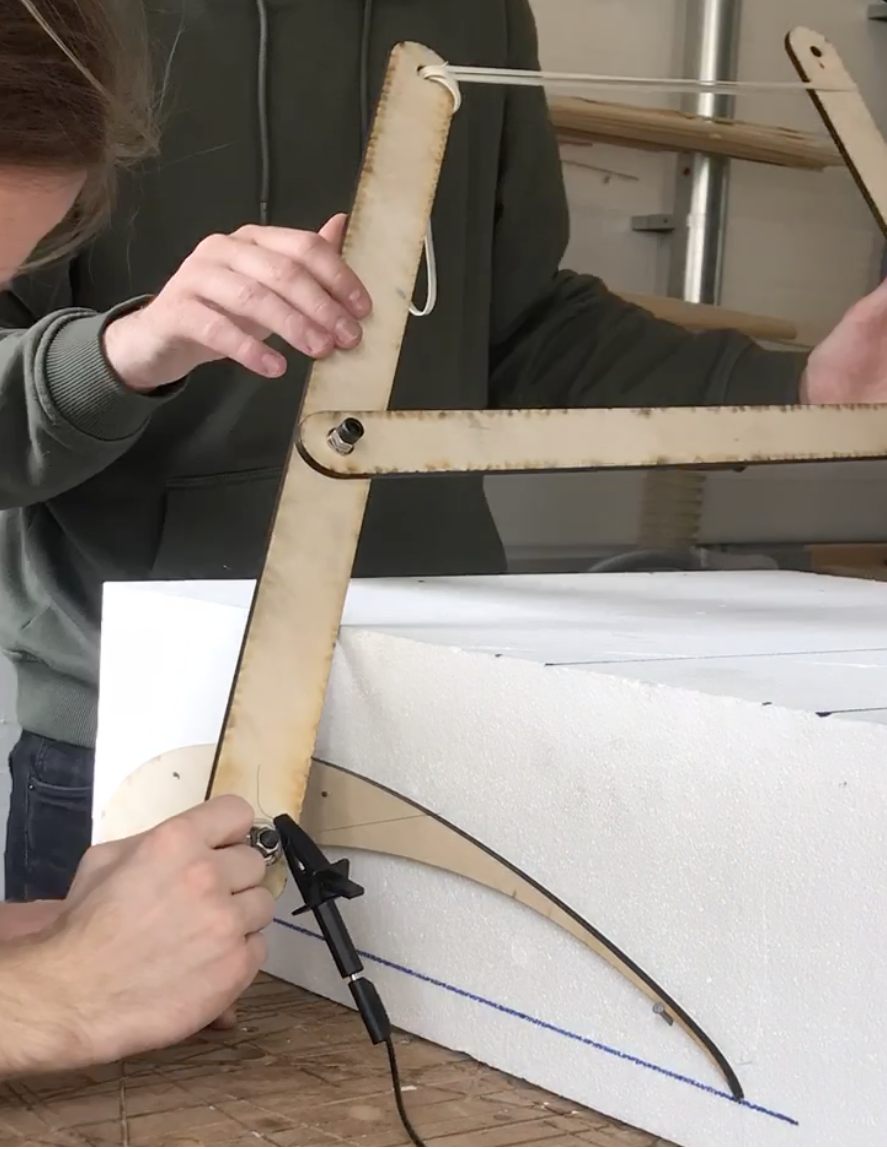
\includegraphics[width=\textwidth]{hotwiremethod}
    \caption{The hot wire melts the styrofoam while sliding along the wooden template.}
    \label{fig:hotwire}
  \end{figure}

  \subsection{Hand Layup}

    \fxnote{Show how we did the hand lay up. What went wrong what went well.}

  \subsection{Surface Finish}

  \subsection{Implementation and Testing}

\section{Testing and Inspection}

  \subsection{Reinforcing the mounting}
